\setcounter{chapter}{ 9 }
\chapter{\textbf{The Tank, Part 1} }



\subChapterTitle{}

\deets{Suko and Adam}{November 8th, 2012}



THE TANK.  Trauma!  Death!  Goo!  Anguish!   Yay!!!!!



As always, please fill in the gaps and correct errors.  Also you should always feel free to add/correct the perspective of your character.


\jumpHeadline{ SAC-09 } 



After seeing Gillian off to Terminus, Hayley boards the train and sees Lackovich already on the train.  She doesn't greet her and moves quietly to the seat furthest away from her.  At Cardoza Station, Oliver boards.  Hayley waves to him. He acknowledges her and goes to sit next to Lackovich.



``Getting back from shore leave?'' asks Oliver.

``Yes,'' Lackovich says shortly.

``I owe you thanks and an apology,'' says Oliver.  Lackovich says nothing.  He continues, ``I wanted to tell you about the Orc of Anglia - you know that name?''

``I was briefed.''

``A lot of shit went down that day, but I won't let him get away with it.''

Lackovich asks him bitterly if that is supposed to make her feel better.

``No, of course not.''

``Then why are you telling me this?''

``I wanted you to know.''



The train returns to SAC-09.  Hayley waits until Lackovich leaves the train, and then she and Oliver disembark and head back to their room.  They find a note from Jonah saying that he's in the lab.  Oliver sits down on his bunk wearily.  Eventually he looks up at Hayley with infinite weariness and says he is going for a swim.  He doesn't ask for company and she doesn't offer.  She does offer to do his laundry though, which he declines.  He goes swimming and Hayley does laundry (hers and Jaya's).



As Oliver is swimming, he hears a knock on the cistern door.  It is Dr. Gerhauser.  She says that she will come pick him up tomorrow.  

``How do you feel?'', she asks.

``A little disappointed, but otherwise intact,'' replies Oliver, which earns him a strange look from Dr. Gerhauser.   She pauses as if she was going to say something and then changes her mind.

``I'm busy tonight,'' she says instead. ``But check in with Swan.  I want you to be in good shape for tomorrow.''

``What's going on tomorrow?''

``You're going in the Tank.  \hl{I thought you should get some warning}\footnote{\textbf{q.google }Really?  How \_considerate\_. \textsubscript{12/07/12 9:50am}}\footnote{$\rightarrow$\textbf{Suko T }This is just Dr. Gerhauser's way of awkward flirting.  It's kinda sweet. :) \textsubscript{12/07/12 11:43am}}.''

``Are you sure you have dinner plans?'' teases Oliver.



That evening, Jari prepares an especially nice meal for Oliver.  Oliver sees Hayley walk into the cafeteria.  She looks around, spots Lackovich and actually turns around and walks back out of the cafeteria.  He gets up and goes to sit with Lackovich and her squad. 



Lackovich is quiet, and Carruthers is too shy to say much, but Oliver's gregariousness draws out the other two and they talk.  Eventually Lackovich gets up abruptly and leaves.  The others linger for a while but eventually leave too.



Oliver runs into Hayley, returning to the cafeteria now that Lackovich is gone.  Hayley asks Jari if there is anything left and he indicates that he'd prepared a small tray.  ``They want you well fed for tomorrow,'' says Jari.

``I am not aware that my nutritional needs had changed,'' says Hayley in surprise, which earns her a short laugh from Jari.  She thanks him for the meal and apologizes for showing up late. He says he has to take care of something in the requisition cage, but she can clean up after herself, right?



Hayley sits in the deserted cafeteria and eats.  Trenton walks in and starts talking to her.  Hayley doesn't leave, but she looks at anything else in the room but him.  He tells her that he's sure she'll do fine tomorrow and rubs her shoulders.  She doesn't pull away but her shoulders do tense.  Desperately Hayley addresses thin air, ``If there is anyone there, please tell Mr. Hadef that I'm not allowed to speak to him.''  When Trenton asks why, she adds, ``Because of orders.'' He seems to find the whole thing amusing and kisses her on the top of her head.  He pauses in the doorway to see if she's watching him, but she's studiously staring in the opposite direction.



Back in their dorm, Oliver is writing a letter.  It takes him a long time and he stares off into space a lot.  Hayley walks in and finds some paper and a pen and starts laboriously writing a letter also.  It is a short message to Trenton.



\textit{``Mr. Hadef.  Please can Signe join you here?  She misses you. She would be a lot of help to you because she knows your work.  Also please check on her, I think she may be unwell.  }\textit{\hl{I am sorry I could not speak to you.  I am under orders not to speak to you or see you}}\footnote{\textbf{q.google }.  This has elements of a Victorian romance ;) \textsubscript{12/07/12 9:54am}}\footnote{$\rightarrow$\textbf{Suko T }I'm thinking more Shakespearean along the lines of a romantic farce. ;P \textsubscript{12/07/12 11:45am}}\textit{. Hayley''}



Hayley tells Oliver that some people want to talk to him because of his father.  But she cannot tell him who wants to talk to him or who told her.  She tells him that it was a Citizen and someone important.  Oliver snaps, ``Really Hayley?  After all that we've been through, you can't tell me?''  Hayley blinks in surprise but doesn't otherwise seem perturbed by his tone.  She  says that her orders on this are very clear.  She can't tell him.



The next morning, they are fed a light breakfast and Rook escorts them to the Tank.  Along the way, Oliver engages Rook in a discussion about the Tank.  \hl{They talk about mind vs body and how the mind controls the body}\footnote{\textbf{q.google }Do any of you remember more about this to elaborate on it?  Just curious, it's not critical. \textsubscript{12/07/12 9:55am}}\footnote{$\rightarrow$\textbf{Suko T }It was actually a decently long conversation.  I'm sorry I didn't take more exact notes.  I think Oliver asked Rook for some more hints on what the Tank was going to be like. \textsubscript{12/07/12 11:58am}}\footnote{$\rightarrow$\textbf{Adam Kenney }Ye-es.  I think Rook was like ``mind over matter, old chap, you'll get through it'' and Oliver was like ``you realize that the brain is part of the body right?''  

I could be misremembering though. \textsubscript{12/08/12 7:25am}}\footnote{$\rightarrow$\textbf{Suko T }That's sounding very likely.  It was definitely along those lines. \textsubscript{12/08/12 11:49pm}}. 



Rook takes them to a room they have not seen before. There is a tank, partially embedded in the floor.  There is a hospital gurney and a table with some familiar items on it (fat cylinders and cap with cables).  The walls are concrete but modified.  There are large cables going into the tank.



Dr. Gerhauser, Swan and Micah are in the room.  Dr. Gerhauser has Oliver sit on the gurney and Swan takes his blood pressure.  Oliver is visibly tense, trying not to crawl out of his skin \hl{as he is forced to submit to authority}\footnote{\textbf{q.google }Right.  Authority.
;) \textsubscript{12/07/12 9:59am}}.  Hayley is taken to the other room by Micah. 



``He looks good, we need to take the Q readings,'' reports Swan.

``I can take care of that, you go take care of Hayley,'' says Dr. Gerhauser. 



When Swan leaves, Oliver relaxes.

``How are you?'' asks Dr. Gerhauser

``Nervous,'' says Oliver honestly.

``Fair enough.  \hl{The important thing is to stay calm.}\footnote{\textbf{Rebecca S. }That's totally not fair! No one gave Jaya this advice! \textsubscript{12/07/12 9:29am}}\footnote{$\rightarrow$\textbf{q.google }Who gives Jaya \_any\_ advice? \textsubscript{12/07/12 10:01am}}\footnote{$\rightarrow$\textbf{Suko T }@Rebecca Heh, Hayley would have, but she was told not to be too helpful. 
@q I dunno, apparently people give Jaya life advice all the time \textsubscript{12/07/12 12:00pm}}\footnote{$\rightarrow$\textbf{Adam Kenney }If someone had told Jaya to stay calm, would she have done it? \textsubscript{12/08/12 7:26am}}''

``Really?  In a war zone, that can sometimes be the wrong reaction.''

``Our literature has several approaches we can try.  We're trying something a little different,'' she says as she places the cap on his head. ``Do you remember the questions from last time?''

``They're a little hazy, I remember the parts of the gun and the area of a triangle.''

``How do you feel about Hayley?''

``Sad.''

``How do you feel about Morgan?''

``Still angry about the Orc of Anglia situation.  Do you talk a lot with her?''

``We're sisters.''

``That doesn't mean anything.''

``We speak quite often.  We don't talk,'' concedes Dr. Gerhauser.



She has Oliver disrobe as she opens the Tank.  ``This is going to feel weird,'' she warns, and she spreads some gel over his face and then puts the mask on.  His face goes a little numb and after a while, he can't feel the mask anymore.

``Any questions?'' asks Dr. Gerhauser.

``No. Let's get this over with.''

She injects him with something else, on the opposite side as last time and indicates that he should climb into the tank.  



\hl{The liquid in the tank feels weird}\footnote{\textbf{q.google }It's interesting that despite Hayley's warnings none of the rest of the team were willing to ask about being drowned. \textsubscript{12/07/12 10:03am}}\footnote{$\rightarrow$\textbf{Adam Kenney }Oliver got some reassurances from someone (Dr. Gerhauser? Agent Rook? Someone else?) about that at some point.  He was told - convincingly or not - that she experienced the sensation of drowning but was not drowned.  Between that and the breathing apparatus - and the fact that at this point Oliver \_has\_ actually drowned in the line of duty, far from medical supervision - he decided it was the least of his problems. \textsubscript{12/08/12 7:28am}}\footnote{$\rightarrow$\textbf{Suko T }+1 
And he was so right.  Apparently lead poisoning was a much greater threat than drowning. :) \textsubscript{12/08/12 11:43pm}}\footnote{$\rightarrow$\textbf{Adam Kenney }I was thinking about what we look like from the perspective of Agent Morgan and Dr. Gerhauser.  Like, we've all acted weird after getting out of the Tank, but a lot of the problematic effects on us have yet to really manifest in ways that are apparent to them.  I think it mainly looks like ``oh, they experienced some disturbing sensations and memories'' rather than ``they are being TORN APART PSYCHOLOGICALLY FROM WITHIN'' at this point.  Do you think they know that's down the road? \textsubscript{12/09/12 9:49am}}\footnote{$\rightarrow$\textbf{Suko T }From Dr. Gerhauser saying ``they are trying some new approaches'' I suspect that they have some idea intellectually, but don't actually comprehend how emotionally traumatizing the situation will be.  They certainly don't have a trained staff psychologist on hand (unless they're being subtle and it's Jari or Tiburon) and it seems like they should if they knew how mentally messed up we were/will be :D \textsubscript{12/09/12 12:26pm}}\footnote{$\rightarrow$\textbf{q.google }''Oliver got some reassurances from someone (Dr. Gerhauser? Agent Rook? Someone else?) about that at some point. He was told - convincingly or not''

I seem to remember a similar conversation between Jonah and Dr. Gerhauser.  I don't think it was reassuring.

``and the fact that at this point Oliver has actually drowned in the line of duty''

That would be reassuring.  Prior knowledge is very useful.  It's hard for those who aren't Citizens or aren't working for them to understand though.  Or at least I've been playing it that way: if the water is really hazardous immersing yourself in it would seem like a crazy idea. \textsubscript{12/10/12 11:40pm}}\footnote{$\rightarrow$\textbf{q.google }''I think it mainly looks like ``oh, they experienced some disturbing sensations and memories'' rather than ``they are being TORN APART PSYCHOLOGICALLY FROM WITHIN'' at this point.
Do you think they know that's down the road?''

``I suspect that they have some idea intellectually, but don't actually comprehend how emotionally traumatizing the situation will be.''

I think they know.  I get the sense they've been through some serious trauma themselves.  They have clearly been working on this project for a long time, and are taking some risks even now.  They behave like people who see the situation they are in as high stakes.  High stakes enough that they are willing to take big risks.  I'm not saying they won't feel any guilt or responsibility, but I think they are probably pretty aware of the risks and the price the patrol might have to pay.  I imagine they see the patrol as just one of the groups making sacrifices \textsubscript{12/10/12 11:45pm}}.  It is definitely more buoyant than regular water.  The Tank hums and Oliver starts sinking.  ``Just let yourself float to the bottom,'' instructs Dr. Gerhauser and then she closes the top of the Tank.



\sceneHeadline{THE TANK: Oliver }

\textit{{[}Trace: 4 Threat Tokens enter the pool{]}}



There is a bright flash of light and suddenly Oliver finds himself in a trench in the Commons where he fought in the war against Nicklepan.  He realizes that this is a memory and yet everything feels so very real that it's hard to entirely believe he's not there.  Everything is incredibly visceral.



\textit{{[}Challenge: Notice 1{]}} There are soldiers around him and he sees that his commanding officer is lying near him, quite dead.  One of his fellow soldiers is yelling at him, but her voice sounds like it is coming from far away.  \textit{{[}Challenge: ``You've been here before'' 2{]}} He notices that all of the sound is somewhat muted, but her voice in particular.  There's an odd sound but he ignores it \textit{{[}Refresh Focused{]}.} He feels as if he is forgetting something, but can't recall what it is.



``Have you heard from Command?  We're going to fucking die here!'' says the other soldier on the verge of hysteria.  Oliver tries to calm her down but she will have none of it, sneering that he'll be fine because he's uninjured but her wounded arm is really messed up and there's no medic.  When he examines his gun, she tells him that it is probably jammed due to all the damn dust.  Oliver fires off the gun just fine and then she says angrily that wealthy guys like him are used to wasting ammo. 



They hear gunfire.  The other soldier says that they need to get out of there.  Oliver looks out of the trench and sees a heavily armored man in Nicklepan colors jump down into a trench nearby. \textit{{[}Challenge: ``Remember where he came from'' 2{]}}.  Oliver realizes that he has never seen the man before and infact those may not even be Nicklepan colors.



Oliver starts to run, dragging the other soldier with him.  One of the walls in the trench collapses and Oliver hears the sound of exploding artillery and popping noises.  The other soldier is wrenched out of his grasp and they are all thrown to the ground.



Oliver gets back up again and realizes that some time has passed.  He is now in a building with a ragtag group of soldiers from various units.  Someone rushes up to Oliver and babbles at him that he's in charge. Oliver flips out and screams at the person that he's not in charge.  \textit{{[}Refresh: Veteran{]} }If they just hang tight the Directorate is sending reinforcements.  ``What the fuck is the Directorate?'' asks the other person.



\textit{{[}Nominal enters the pool.  8 threat tokens{]}}



Time seems to hiccup again and the situation changes.  \textit{{[}Challenge: Notice 1{]} }Oliver sees that the others around him are listless and tired.  He also realizes that he is having trouble breathing.  Oliver decides to bring his focus inward and steadies his breathing \textit{{[}Refresh: Focused{]} }at the expense of noticing what is going on around him.  



He misses Nicklepan's next push and when he is aware again, he is being shot at from above.  He is lying near a wall, entirely exposed.  The nearest cover is the subway entrance. He knows there are people down there, but right now he can't remember if they are friend or foe.  Oliver realizes that his leg is still whole and hale, and leaps for the entrance as a smattering of gunfire hits where he was.  It is thrilling to be able to move like that again.



Oliver goes down into the subway.  He hears movement and the sound of a train coming.  He sees a gun nest, being manned by Nicklepan soldiers. \textit{{[}Challenge: Gun down Nicklepan soldiers 3{]}}.  Oliver easily dispatches them with a clean headshot each.



The train comes into the station, but before Oliver can get there, he runs into another soldier shooting at him. \textit{{[}Challenge: Avoid getting shot 2{]}}.  Oliver doesn't flinch and dives for cover in the gun nest.



The train doors open and Oliver lays down covering fire for them. \textit{{[}Challenge: Give cover{]}}.  A tall woman walks up to him.  Flanking her is a medic, Jonah, and a Fili, Judi.  The woman demands to know who is in command and what is going on.

``Are you injured?'' Jonah asks.

``No, but I will be.''



Oliver freaks out {[}\textit{Refresh: Hardened}{]} and Jonah shouts, ``We've got a headcase here!''

``What's your name?'' asks Jonah.

``Constable Oliver Langdon,'' replies Oliver.

``There are no Constables here.  Just calm down,'' says Jonah soothingly.



\textit{{[}Challenge: Notice insignia 1{]}}  As Oliver looks at Jonah, he realizes that the insignia on Jonah's collar isn't right.

``Where are we?'' asks Oliver. 

``Do \textit{you }know where we are?'' counters Jonah.  \textit{{[}Challenge: Answer correctly 2{]}}

``We're at Curiosity Ridge,'' replies Oliver and then feels sense of dissociation and a presence behind his eyes, somewhere where he can't see it.



\textit{{[}Solid enters the pool.  12 threat tokens added{]}}



Oliver sees Ogleby, leading a ragtag group of people.  He's exhorting them to retake Transit Minor.  Oliver realizes that his leg is still okay but he's near DX Station.  \textit{{[}Challenge: Notice 1{]}}  Oliver addresses Ogleby as Senior Constable.  Ogleby indicates that they are going to have to run through the Kill Zone that Oliver remembers so well.



Oliver backs away discreetly and then deserts. \textit{{[}Refresh: Veteran{]} {[}Challenge: Avoid anyone noticing the desertion 3{]}} Oliver makes it to some of the side streets and is creeping through the shadows when he comes across a soldier in one of the alleys.  Oliver claims he's being sent to get into sniping position, but the soldier challenges him - saying he knows a deserter when he sees one. \textit{{[}Challenge: Kill the guy 3{]}}



Oliver shoots the guy in the head, but then freaks out a little \textit{{[}Refresh: Focused{]}}. A figure in dark body armor drops down. ``What the hell you'd do that for?'' she asks.  ``It was a mistake, I thought he was an enemy,'' claims Oliver.  The figure steps forward.  ``Do you trust me?''  \textit{{[}Challenge: See face 2{]}} Oliver sees the face behind the helmet visor and realizes that it is Morgan.



Morgan snaps her rifle up and points it at Oliver.  ``You're not supposed to be here,'' she says.

``Neither are you,'' Oliver replies.  ``I trust you.'' The butt of the rifle swings around and Oliver feels intense pain as it connects with his head.



He wakes up in the mud.  Ogleby pulls him to his feet. \textit{{[}Challenge: Push through the pain 2{]}}. Even though he has a blinding headache, Oliver staggers to his feet and checks his gun. \textit{{[}Refresh: Crack Shot{]}}



Another soldier tries to drag Oliver out into the street, yelling at everyone to press on.  ``Come on Martoni, you redheaded bastard!  MOVE!''  \textit{{[}Challenge: Avoid getting dragged out into the street 2{]}.  }



Oliver points out how exposed they will be running down the middle of the street {[}\textit{Challenge: Impress the guy 3}{]} and convinces him to get out of the street.  



Oliver stares down at his gun in confusion.  ``This isn't my gun!'' he says and throws it down {[}\textit{Refresh: Firearm: Sniper Rifle}{]}

Oliver sees that Ogleby has a sniper rifle (or something that looks like one).  Unfortunately Ogleby is across the street.  Oliver runs across the street \textit{{[}Refresh: Hardened{]}}.  As he runs, he sees That Building and sees That Flash of Light.



\textit{{[}Challenge: Avoid getting shot 4{]}} There is a brief moment of pain in both his hand and his leg and Oliver blacks out.



\textit{\textbf{{[}6 tokens left on Solid for Oliver{]}}}


\sceneHeadline{\hl{THE TANK: Hayley} }\footnote{\textbf{q.google }Saving Hayley's Tank writeup for last is \_exactly\_ the right order to experience the Tank! \textsubscript{12/07/12 10:33am}}

Hayley's prep goes much faster.  She eagerly assists Swan in prepping herself for the Tank.  She doesn't get asked questions like Oliver did.  Dr. Gerhauser just does some basic checks before they knock Hayley out and put her in the tank.



Hayley wakes up.  The air/goo she is suspended in seems brighter than before and slightly pinkish, but still hazy and strange.  She feels sluggish and odd.  She holds her breath for a while but then trusts in Dr. Gerhauser and takes a deep breath.  \hl{She finds she can breathe but it is difficult}\footnote{\textbf{q.google }So is Hayley not wearing a mask? \textsubscript{12/07/12 10:10am}}\footnote{$\rightarrow$\textbf{Suko T }It was my impression that no, she is not wearing a mask when she wakes up in the ``other'' tank.

Whether or not she's wearing one when they dunk her in the tank on the SAC-09 side is unknown since they knocked her out both times before she's been put in the tank. \textsubscript{12/07/12 12:02pm}}\footnote{$\rightarrow$\textbf{q.google }Yeah when I re-read it I realized we don't really know.  Go ambiguity :). \textsubscript{12/11/12 8:09pm}}\footnote{$\rightarrow$\textbf{Suko T }I think it's reasonably clear on the non SAC-09 side.  When she climbed out of the tank she vomits up goo and wipes it off her face with no mention of ``removing the mask first''.  If she didn't have a mask, why would she have inhaled goo?  So I expect that it was all like in the Abyss and she was breathing oxygenated liquid.  That's how I pictured the whole scene anyway.  Which will likely freak out Jonah even more than just being submerged :D

On the SAC-09 side, she didn't remove a mask to speak to Swan when she climbed out, but she also didn't cough up goo to clear her lungs either, so perhaps it's just a detail that was skipped. \textsubscript{12/13/12 5:23pm}}. \textit{{[}Challenge: Difficulty Breathing 1{]}}



She bangs her head on something metallic above her.  She feels around and tries to peer through the glass wall around her.  She can see someone looking back at her.  \textit{{[}Challenge: Notice woman 1{]}}.  It is a woman with blond hair, her eyes have burst blood vessels in them and her mouth hangs open slackly.  She looks dead.  Seeing the blond hair reminds Hayley of her last experience and she tries to see what color her hair is.  She realizes that she is bald.  No surgery scars though.  Being bald upsets her more than being suspended in goo.



She tries to knock on the glass but can only manage a feeble tapping.  She feels around on the metal ``ceiling'' and eventually finds some handles.  \textit{{[}Challenge: Open tank 2{]}}  With effort and some gymnastic contortions, Hayley manages to pull the handles down.  The lid to the tank opens and the liquid begins to slowly drain out of the tank.



Hayley clings to the edge of the tank, wiping the goo off of her face and vomiting up more of the liquid.  Once she can breathe again she climbs out of the tank.



The tank is partially submerged into the floor.  There are multiple tanks and there are metal catwalks between them.  There are two doors, one on each side of the room.  They are both closed.



Hayley goes over to the tank with the blond woman.  The liquid around her is darker than in Hayley's tank.  The woman's hand looks mangled and there is a cloud of darker liquid around it.  As Hayley looks at her, she is overwhelmed with emotion.  \textit{{[}Challenge: Don't freak out 3{]}}  Hayley loses it, first sobbing uncontrollably, and then screaming in anguish.  \textit{{[}Refresh: Conditioned{]}} She frantically wrenches the tank open and pulls the woman out.  When the tank opens, there is a strong stench of rot and decay. The woman is clearly dead.



\textit{{[}Challenge: Notice potential threat 1{]}} Hayley senses some vibrations in the floor and blindly turns to face the new threat, her body protectively braced over the dead woman.  She can see no one.  After arranging the woman's body carefully in a decorous way, Hayley goes scouting.  



\hl{She passes another tank with a broad shouldered man in it.  The tank across from him is almost completely black.   It looks like there may be something in there, but she can't see what it is.  There are two more tanks, one with a woman and the other with a man.  The man is twitching.}\footnote{\textbf{Rebecca S. }!!!! \textsubscript{12/07/12 10:11am}}\footnote{$\rightarrow$\textbf{q.google }!!!! !!!! \textsubscript{12/07/12 10:21am}}\footnote{$\rightarrow$\textbf{Nathaniel Ford }!!!

? \textsubscript{12/24/12 7:07pm}} 



She goes to the door closest to her.  \textit{{[}Challenge: Notice 1{]}}  There are two panels next to it.  There is a window that is lit purple.  Hayley stabs at the buttons randomly, but nothing seems to happen.  She tries to batter the door down but it is far too solid.



Hayley starts yelling for help. \textit{{[}Challenge: Notice 1{]}}  She pounds on the tank with the guy who is twitching.  He stops twitching for a few moments, but then starts twitching again.



She notices that there are lockers next to the tanks. She opens the locker next to her tank and finds a strange looking suit/uniform inside, some sealed packages and a picture of the blond woman in a sundress.



While she is looking at the photo, the other door opens.  Hayley instinctively moves to interpose her body between whomever is coming through the door and the dead woman.



The figure opens fire and \textit{{[}Challenge: Avoid gunfire 3{]}} Hayley charges at her attacker, hardly slowing as flechettes strike her painfully.  The shooter is a pale man in a jumpsuit.  He is short.  He drops the gun and braces to meet her charge.  Out of her mind with protective rage, Hayley rushes at him, snarling and cursing like a...Jaya.  \textit{{[}Refresh: Protocol{]}}



He tries to grab her, but she slips and ends up sprawling right at his feet \textit{{[}Refresh: Athletics{]}}.  He starts choking her with ungodly strong hands. \textit{{[}Challenge: Stop being choked 4{]}  {[}Challenge: Notice 2{]}}



Hayley suddenly is back in the Tank.  She remembers her throat being crushed, and the excruciating pain, but can disassociate herself from it.  



She feels around on the Tank ceiling.  It feels different than the one before, but she finds something that seems like a handle and yanks on it.  The tank lid opens and Swan is reaching in to help her out.  ``That was really fast, is everything ok?'' he asks.  As soon as Hayley can speak, she says, ``I don't think I did that well.  Can I try it again?''



Swan says he has to ask to Dr. Gerhauser.  He helps Hayley over to the gurney and asks her what happened.  He takes notes as she describes what she saw.  He draws pictures and diagrams and mocks up a system of various weights so that Hayley can demonstrate how much effort it took to open the tank lid.



Dr. Gerhauser comes in during Hayley's report and mostly just listens, occasionally asking a clarifying question.  When Hayley starts to describe the woman, Hayley tears up and cannot speak for a few moments.  She describes the woman's broken hand and that she was dead.  When they asked why she pulled the woman out of the tank, Hayley replies that she was hoping that the woman could be revived. After all, they brought back Oliver from death, didn't they?  Hayley mentions that the woman was very beautiful in the photograph.  They ask her about the photo and she describes the other contents of the locker she found it in.



As her emotional equilibrium comes back, Hayley mentions that she had no hair.  She describes the other people in the other tanks.  Dr. Gerhauser goes pale when she mentions the twitching man.



\textit{{[}Ongoing Challenge: The Tank $\rightarrow$ Athletics 2 (Hayley){]}}



Hayley asks to try again but is refused.  She asks what she can do better next time, and is told that getting names would be good, and as many details as she can learn.



Hayley says she does not want the others to have to go through the Tank.  She is concerned over Oliver, getting very distressed when she learns he is already in the Tank.  Dr. Gerhauser discharges Hayley to return to the dorm, and assures her that Oliver is okay and sleeping in Medbay.  ``He came out suddenly, like you did.  \hl{He is not as acclimated as you are to this kind of thing}\footnote{\textbf{q.google }\_shudder\_ \textsubscript{12/07/12 10:23am}}.''



Hayley asks if she can go in the Tank for him.  Dr. Gerhauser says instead, ``I am going to need your help with something.''

``Yes, whatever you want,'' says Hayley eagerly.

Dr. Gerhauser pauses and gently admonishes, ``You should be careful when you say that.''

Hayley looks at her uncomprehendingly and says, ``OK.''

Dr. Gerhauser continues, ``Your patrol group is good at certain things.''

\hl{``We are??'' says Hayley incredulously.}\footnote{\textbf{Rebecca S. }:) Jesus, Hayley, have a bit more faith in your team! Respect, woman! Respect! \textsubscript{12/07/12 10:15am}}\footnote{$\rightarrow$\textbf{q.google }We are actually.  Although my list is different than Dr. G's. \textsubscript{12/07/12 10:23am}}\footnote{$\rightarrow$\textbf{Suko T }There was a taste of it in Jaya's tank scene, but probably is best that no one asks Hayley what she really thinks of the team... :D \textsubscript{12/07/12 12:04pm}}

``Yes.  Oliver is good at shooting people, Jonah is an excellent field medic, and I wouldn't want to run into Jaya in a dark alley.  \hl{But you are better at \textit{this}, and are going to be for some time}\footnote{\textbf{q.google }Yeah.  Hayley is clearly on a very different plane than the rest of us.  Her use of the tank seems much closer to its intended purpose.

(I'm a little disturbed about what this says about the upsides of being abused your whole life....) \textsubscript{12/07/12 10:25am}}.  They have to learn it on their own.''



Dr. Gerhauser lays out some rules for Hayley.  Don't discuss it overmuch with them.  Let them work through it.  She can tell them what she saw, but they have to do it and process it on their own. \hl{She can't help them with that}\footnote{\textbf{q.google }It seems unfortunate until you realize that she really can't: None of them will listen, not until they've actually begun to figure it all out anyway.  I don't even think it's just that Hayley's explanations are coming from an angle the others don't completely understand, or even that all of them are stubborn and defensive -- both of which are true.  I think it's more fundamental to human nature, or at least to how people learn things.  This is too alien an experience for the verbal preparation to do much. \textsubscript{12/07/12 10:29am}}\footnote{$\rightarrow$\textbf{Suko T }+1 \textsubscript{12/07/12 12:07pm}}.  ``Oliver has had his first experience and it's going to take him awhile to figure out where it fits.''  Protocol-sensitive Hayley notes the use of Oliver's first name, but says nothing.



``What \textit{is} this?'' Hayley asks, confused.

``\hl{This is a very old take on a very new thing}\footnote{\textbf{q.google }\_Huh\_.  I was thinking the it was a very new take on a very old thing!  I'll have to watch this more carefully. \textsubscript{12/07/12 10:27am}}.''

When Hayley asks if Dr. Gerhauser will give a lecture on the Tank, she says that she might, once everyone reaches a certain level of understanding on their own.





Hayley is still agitated, and Dr. Gerhauser says, ``You should remember that it's not actually you.  Remember when you broke your hand?''

It takes a while but Hayley eventually puts 2 and 2 together and realizes that she must have been the blond woman last time.  This upsets her.  ``Do I always go back to the same place?''

\hl{``This time, we believe you did, yes,}\footnote{\textbf{q.google }!!!!

I am \_so\_ glad I hadn't read this when we played yesterday! \textsubscript{12/07/12 10:35am}}\footnote{$\rightarrow$\textbf{Rebecca S. }I gotta' say : ``Called it!'' \textsubscript{12/07/12 11:32am}}\footnote{$\rightarrow$\textbf{Suko T }Yes it was pretty clear why Nate specifically asked that these notes not be shared until after your tank sessions. \textsubscript{12/07/12 12:08pm}}\footnote{$\rightarrow$\textbf{Adam Kenney }Rebecca, what was your theory? \textsubscript{12/08/12 7:31am}}\footnote{$\rightarrow$\textbf{Rebecca S. }The tank experience is our team mentally transporting into other bodies. Unclear of where these bodies are in time \& space.  That non-Hayley tank scenes are just us trying to mentally work our way to the ``surface''.  My opinion remains un-changed since the first tank scene \& our meeting other Tankians on that drowned mission.  I'm hoping at some point we figure out that the Tankian Jaya took prisoner is actually one of the TA team in tank mode. \textsubscript{12/27/12 8:32pm}}`` says Dr. Gerhauser.

``Is that supposed to happen?  Will I die everytime I go back?''

``The first time you went into the Tank, we had a short window of opportunity.  The woman was going to die anyway.  It may be best not to mention those things to your squadmates.''  Dr. Gerhauser adds with unexpected gentleness, ``would you like to stay in Medbay tonight?''

Hayley nods.  ``Yes please.  I feel safer here.'' 

``Are you alright?'' asks Dr. Gerhauser.

``No,'' says Hayley frankly.

``Do you believe that you'll be willing to proceed in the future?''

``Yes.  As soon as possible, please,'' says Hayley just as promptly.



Hayley thinks for a moment.  ``We have to figure this out....right?  Then no one else will ever need to do it?''

Dr. Gerhauser doesn't address the question directly, instead replying, ``We believe we will reach a point where your whole group will need to do this together.''



Hayley apologizes for failing the test.  

``Why do you think you failed?  You shouldn't be so hard on yourself.  The first time you thought you failed.  This time you got much further and you still think you failed.  What would you have considered a success?  If you made it down the corridor?  Or something else?'' asks Dr. Gerhauser curiously.

\hl{``I would succeed when I reach the end.  When I win,'' says Hayley, bewildered.

``There is no end to anything.  You should come to terms with that,'' says Dr. Gerhauser.}\footnote{\textbf{q.google }This by far my favorite conversation in the whole game. \textsubscript{12/07/12 10:36am}}\footnote{$\rightarrow$\textbf{Suko T }It really hit Hayley in one of her vulnerable spots. \textsubscript{12/07/12 12:11pm}}\footnote{$\rightarrow$\textbf{q.google }I'm actually surprised to learn Hayley is motivated by the notion of winning.  I thought she thought she failed because she didn't follow orders properly (whatever her orders were). \textsubscript{12/11/12 8:15pm}}\footnote{$\rightarrow$\textbf{Suko T }It's less ``winning for the sake of victory'' than for ``winning/finishing means it's done and I know my place in the world.''  Hayley is very ``concrete goal''-driven, so when someone tells her that there is no goal to strive for, it freaks her out worse than 5 year olds being told there is no Santa.  If there is no end goal to tell her when she's finished something, how can she know how well she did? Chaos and uncertainty terrify her.  And she has to do ``her very best''.  It's very Dollhouse.  The drive to ace anything that seems like a test is VERY strong. \textsubscript{12/12/12 11:02am}}\footnote{$\rightarrow$\textbf{Suko T }Oh and as for the: ``I thought she thought she failed because she didn't follow orders properly (whatever her orders were).''  

It's not that, because you've seen what she does when she thinks she hasn't followed orders (like with Trenton) or if she thinks the orders she was given were unclear/flawed.  It's a very different sort of reaction. \textsubscript{12/13/12 5:28pm}}



This upsets Hayley greatly and her knuckles turn white as she grips the edge of the gurney.  Dr. Gerhauser stops questioning Hayley and says that perhaps she should rest now.  Hayley is very agitated and pleads to see Constable Langdon.  She just needs to see that he's okay.  Dr. Gerhauser leads Hayley to the room where Oliver is sleeping peacefully.  Hayley watches him breathe for a few seconds and listens to the machines softly beeping.  Much of her previous tension drains away.  She thanks Dr. Gerhauser and seems much calmer as she settles into her Medbay room. 


\sceneHeadline{Oliver \& Dr. Gerhauser }

Oliver wakes up in Medbay.  He can see a figure sitting next to a lamp.  He has a splitting headache.



The figure speaks, it is Dr. Gerhauser.  She pulls up a chair and turns down the light when he says it is too bright.  



``Were you in the war?'' asks Oliver.

``Which war?''

``Nicklepan.''

``No''

``What about Caldonia?''

``Where did you hear that name?'' asks Dr. Gerhauser sharply.

\hl{``Guess.''}\footnote{\textbf{q.google }Ha! \textsubscript{12/07/12 10:37am}}

``Yes,'' says Dr. Gerhauser.  ``Morgan and I come from Caldonia.  Well New Caldonia to be more accurate.  It was destroyed.''

``Where is it?''

``It is very far away.''

``How did you get here?''

``It is a long story.''

``I have nowhere to go,'' says Oliver, wryly.

``Perhaps I misspoke.  It is a painful story.  Morgan and I fled and ended up here, where \hl{Morgan was able to work her magic}\footnote{\textbf{q.google }Wait.  Hecate... Morgan(na?)... 

He said there were no \_psionics\_ in the game but he said nothing about magic. \textsubscript{12/07/12 10:39am}}\footnote{$\rightarrow$\textbf{Nathaniel Ford }Sufficiently advanced technology and all... \textsubscript{12/24/12 7:11pm}}.''

``Who were you fighting?''

``You know them as Anglia. Why do you want to know?''

``I'm not sure what war I was fighting in.  Morgan was there.  They kept calling me 'Caldonian redhead Martoni'.''

``You were referred to as Martoni?''

``Yeah''

Dr. Gerhauser thinks for a moment.  ``I'll tell my sister that you want to bow out of the experiment, if you want.  If you don't, you will have to work through it.''

``\hl{Why are you giving me a choice now}\footnote{\textbf{q.google }Why is she giving Oliver a choice at all?  Don't tell Jonah there's a choice...

Also, does this strike anyone else as trying to change the subject, or at least that Oliver got a little too close to something sensitive? \textsubscript{12/07/12 10:41am}}\footnote{$\rightarrow$\textbf{Suko T }I got more of the sense that she was remembering how she was forced to do something she didn't want to do and how unhappy she was about it, and maybe out of sympathy/empathy was giving him an ``out''.   Could be wrong though. \textsubscript{12/07/12 12:14pm}}\footnote{$\rightarrow$\textbf{Adam Kenney }I got a similar sense to what Suko said, with a slight twist: maybe she knew Martoni and knew what happened to him, or what he did, and didn't want Oliver to experience that. \textsubscript{12/08/12 7:39am}}\footnote{$\rightarrow$\textbf{Suko T }OOo!  I can see that now.  That would be cool. \textsubscript{12/08/12 11:42pm}}?''

``You had to have a taste.  I believe that you should not make a decision without knowing what it is like.''

``What the point of it?  What am I supposed to accomplish?''

``Familiarity.  I can tell you things and add layers on top of the experience, but that will only inhibit your ability to get familiar with it.  You'll know when you get it.  You haven't got it yet.''  Dr. Gerhauser.

Oliver laughs and then winces in pain.  ``Ow!  Stop making me laugh.''

Dr. Gerhauser says, ``I'm glad you are awake but you should rest now.''



Oliver starts drifting off.  Just as he passes out, he thinks that she touches his hand lightly.  There is the spark of electricity from human contact, but also a sensation of burning.  Oliver feels a presence behind his eyes as he slips into unconsciousness.



\jumpHeadline{Challenges \& Refreshes } 

{
\parskip=0pt
\begin{itemize}
\item Challenge: Notice 1.  Focused 2 (Oliver) $\rightarrow$ Overcome! \textbf{1 VP (Oliver)}
\item Challenge: Notice ``You've been here before'' 2.  Veteran 2 $\rightarrow$ Matched
\item Refresh: Focused (Oliver)
\item Challenge: ``Remember where he came from'' 2.  Focused 2 (Oliver) + \textbf{ {\color[RGB]{255,0,0}Flaw: Nightmares 2{[}0{]}} } $\rightarrow$ Overcome! \textbf{2 VP (Oliver)}
\end{itemize}

\begin{itemize}
\item Refresh: Veteran (Oliver)
\end{itemize}

\begin{itemize}
\item Challenge: Notice 1.  Outgoing 2 (Oliver) $\rightarrow$ Overcome! \textbf{1 VP (Oliver)}
\end{itemize}

\begin{itemize}
\item Refresh: Focused (Oliver)
\end{itemize}

\begin{itemize}
\item Challenge: Gun down Nicklepan soldiers 3.  Crack Shot 3 (Oliver) $\rightarrow$ Matched
\item Challenge: Avoid getting shot 2.  Hardened 3 (Oliver) $\rightarrow$ Overcome! \textbf{2 VP (Oliver)}
\item Challenge: Give Cover 2.  Firearms: Sniper Rifle 2 (Oliver) $\rightarrow$ Matched
\item Refresh: Hardened (Oliver)
\item Challenge: Notice insignia 1. Citizen 1 (Oliver)  $\rightarrow$ Matched
\item Challenge: Answer correctly 2. Veteran 2 (Oliver)  $\rightarrow$ Matched
\item Challenge: Notice 1 $\rightarrow$ Sent back to pool
\item Refresh: Veteran (Oliver)
\item Challenge: Avoid anyone noticing the desertion 3.  Focused 2 (Oliver) $\rightarrow$ Sent back to pool
\item Challenge: Kill the guy 3. Hardened 3 (Oliver) $\rightarrow$ Matched
\item Refresh: Focused (Oliver)
\item Challenge: See face 2.  Focused 2 (Oliver) $\rightarrow$ Matched
\item Challenge: Push through the pain 2.  Hardened 3 (Oliver) $\rightarrow$ Overcome! \textbf{2 VP (Oliver)}
\item Refresh: Crack Shot (Oliver)
\item Challenge: Avoid getting dragged out into the street 2. Anti-Authoritarian 1 (Oliver) + Arm Strength 1 (Oliver) $\rightarrow$ Matched
\item Challenge: Impress the guy 3. Veteran 2 (Oliver) + \textbf{ {\color[RGB]{255,0,0}Flaw: Insecurity about war history 2{[}0{]} } } $\rightarrow$ Matched
\item Refresh: Firearm: Sniper Rifle (Oliver)
\item Refresh: Hardened (Oliver)
\item Challenge: Avoid getting shot 4 $\rightarrow$ Sent back to pool
\item Challenge: Difficulty Breathing 1.  Conditioned 2 (Hayley) $\rightarrow$ Overcome! \textbf{1 VP (Hayley)}
\item Challenge: Notice woman 1.  Lady's maid 2 (Hayley) $\rightarrow$ Overcome! \textbf{1 VP (Hayley)}
\item Challenge: Open Tank 2.  Athletics 2 (Hayley) $\rightarrow$ Matched 
\item Challenge: Don't freak out 3.  Protocol 1 (Hayley) + Unashamed 1 (Hayley) + \textbf{ {\color[RGB]{255,0,0}Flaw: Fear of anyone she deeply cares about using the Tank 2{[}0{]}} } $\rightarrow$ Matched 
\item Refresh: Conditioned (Hayley)
\item Challenge: Notice potential threat 1.  Bodyguard 1 (Hayley) $\rightarrow$ Matched 
\end{itemize}

\begin{itemize}
\item Challenge: Notice 1.  $\rightarrow$ Sent back to pool
\item Challenge: Notice 1.  $\rightarrow$ Sent back to pool
\end{itemize}

\begin{itemize}
\item Challenge: Avoid gunfire 3. Conditioned 2 (Hayley) $\rightarrow$ Sent back to pool
\item Refresh: Protocol (Hayley)
\item Refresh: Athletics 2 (Hayley)
\item Challenge: Stop being choked 4 $\rightarrow$ Sent back to pool
\item Challenge: Notice 2. Gorgeous 3 (Hayley) $\rightarrow$ Overcome! \textbf{2 VP (Hayley)} 
\end{itemize}
}


\jumpHeadline{Ongoing Challenges }  

\begin{itemize}
\item Ongoing Challenge: The Tank $\rightarrow$ Athletics 2 (Hayley)
\item (possibly) Ongoing Challenge: The Tank $\rightarrow$ Hardened 3 (Oliver)
\end{itemize}



\jumpHeadline{ Tank Challenge Levels }  

{
\parskip=0pt
Trace: Green

Nominal: Yellow

Solid: Orange

Synchronous: Red
}


\jumpHeadline{ VP TOTALS } 

{\parskip=0pt
Hayley 4

Oliver 8
}


\jumpHeadline{ Quotes }  


\quotedDialog{
``How do you feel?'' 

``A little disappointed, but otherwise intact.'' -Adam as Oliver
}
\extraIndent{- Dr. Gerhauser and Oliver}



``We speak quite often.  We don't talk.''

\extraIndent{- Dr. Gerhauser}


\quotedDialog{
``Your patrol group is good at certain things.'' 

``We \textit{are}??''
}
\extraIndent{- Dr. Gerhauser and Hayley }


\quotedDialog{
\hl{``Are you alright?'' 

``No.''

``Do you believe that you'll be willing to proceed in the future?''

``Yes.  As soon as possible, please.''}\footnote{\textbf{Suko T }I feel this sums up Hayley so well. \textsubscript{11/10/12 3:48am}}
}
\extraIndent{- Dr. Gerhauser and Hayley }


\quotedDialog{
``Do I always go back to the same place?''

``This time, we believe you did, yes.''

``Is that supposed to happen?  Will I die everytime I go back?''

``The first time you went into the Tank, we had a short window of opportunity.  The woman was going to die anyway.  It may be best not to mention those things to your squadmates.''
}
\extraIndent{- Hayley and Dr. Gerhauser}

%\vspace{\fill}

\begin{flushright}
\textsubscript{last edited by \textbf{Nathaniel Ford} @ 05/07/15 4:28pm}
% Exported @ 08/23/15 10:27pm
\end{flushright}

\begin{flushright}
~
\vskip 15em
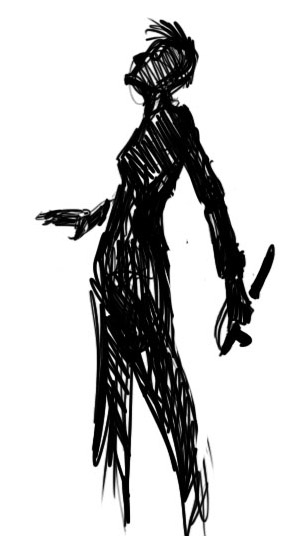
\includegraphics[width=6cm]{img/book1_jaya_stand_misc.jpg}
\end{flushright}
